\chapter{XAI-Auswertung}\label{chap:XAI-Methoden}

Dieses Kapitel untersucht, welche Merkmale die Modellentscheidungen erklären. Dafür werden globale und lokale XAI-Methoden kombiniert. Die globale Sicht zeigt, welche Merkmale das Modell insgesamt stark nutzt. Die lokale Sicht zeigt dagegen, wie eine einzelne Vorhersage zustande kommt.

Als erklärtes Modell wurde der Random Forest verwendet. Das MLP erreicht im Modellvergleich zwar den höchsten Macro-F1-Wert, liegt aber nur knapp vor den anderen Modellen. Für die XAI-Auswertung ist der Random Forest deshalb ein sinnvoller Kompromiss: Er erreicht mit einem Macro-F1 von 0{,}931 fast dieselbe Leistung wie das MLP, arbeitet direkt auf den unskalierten Merkmalen und ist als baumbasiertes Modell gut mit TreeSHAP erklärbar \cite[Kap.~18]{molnar2025interpretable}. Die Erklärung bezieht sich also nicht auf das formal beste Modell des Testlaufs, sondern auf ein ähnlich leistungsstarkes Modell, dessen Entscheidungen besser auswertbar sind.

Die Auswertung verwendet drei Methoden: Permutation Feature Importance, SHAP und LIME. Permutation Feature Importance dient als globale, leistungsbezogene Erklärung. SHAP wird global und lokal genutzt. LIME ergänzt die lokale Betrachtung durch ein zweites, anders aufgebautes Erklärungsverfahren. Diese Auswahl passt zur in Kapitel~\ref{chap:Grundlagen} beschriebenen Zielsetzung: Die Erklärungen sollen nicht nur technische Ranglisten liefern, sondern zeigen, ob das Modell nachvollziehbare Größen- und Forminformationen verwendet.

\section{Globale Erklärungen mit Permutation Feature Importance}

Permutation Feature Importance misst, wie stark die Modellleistung sinkt, wenn die Werte eines Merkmals zufällig vertauscht werden. In dieser Arbeit wurde dafür der Macro-F1-Score auf den Testdaten verwendet. Das ist konsistent mit der Modellbewertung aus Kapitel~\ref{chap:Ergebnisse-der-Klassifikation}, weil die Klassen im Datensatz ungleich verteilt sind.

Abbildung~\ref{fig:Permutation_Importance_RandomForest} zeigt die globale Rangfolge. Am wichtigsten ist \texttt{ShapeFactor1}. Danach folgen \texttt{Roundness}, \texttt{Area} und \texttt{Compactness}. Die beiden Merkmale \texttt{AspectRatio} und \texttt{Eccentricity} liegen deutlich niedriger. Für den Random Forest bedeutet das: Wird die Information aus \texttt{ShapeFactor1} zerstört, verliert das Modell im Testset am meisten Macro-F1. Wird dagegen \texttt{Eccentricity} permutiert, verändert sich die Leistung nur wenig.

\begin{figure}[htbp]
  \centering
  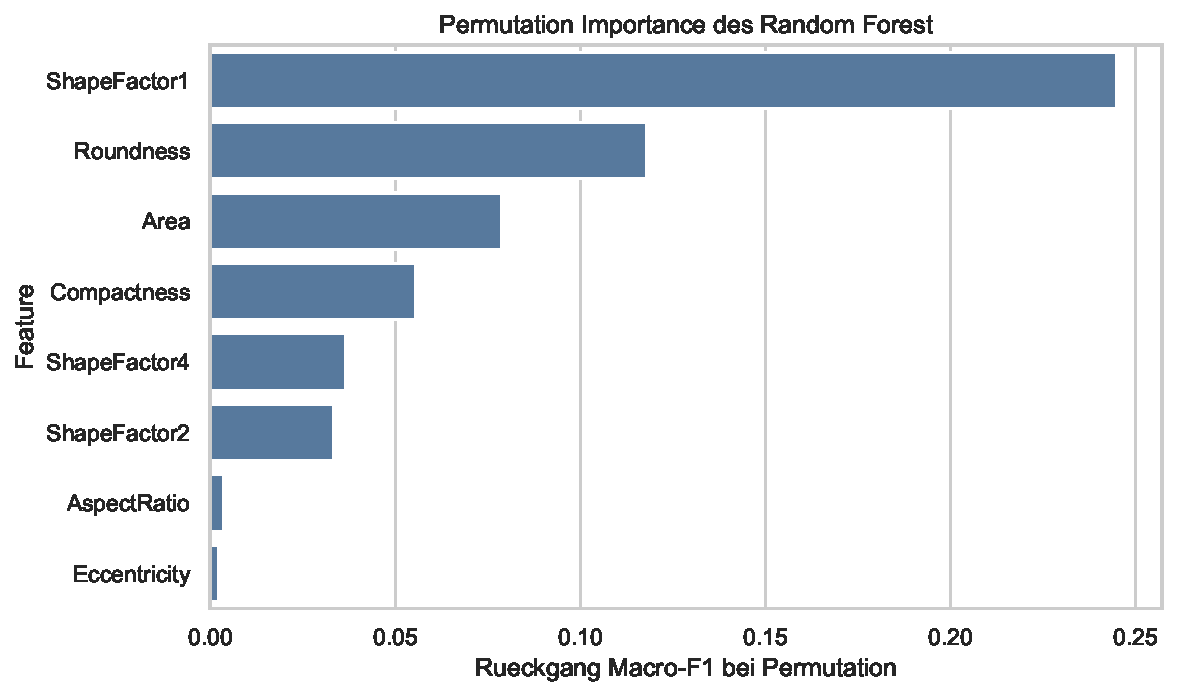
\includegraphics[width=0.85\textwidth]{Graphics/Permutation_Importance_RandomForest.pdf}
  \caption{Permutation Feature Importance des Random Forest}
  \label{fig:Permutation_Importance_RandomForest}
\end{figure}

Die Rangfolge ist fachlich plausibel. \texttt{ShapeFactor1}, \texttt{Roundness}, \texttt{Area} und \texttt{Compactness} beschreiben Größe und Form der Bohnen. Genau diese Eigenschaften sind für eine Sortenerkennung naheliegend. Gleichzeitig muss die PFI vorsichtig gelesen werden. Molnar weist darauf hin, dass PFI bei korrelierten Merkmalen unrealistische Datenpunkte erzeugen kann und nur den Leistungsverlust zeigt, nicht die Richtung des Effekts \cite[Kap.~23]{molnar2025interpretable}. Für den Dry-Bean-Datensatz ist diese Einschränkung relevant, weil mehrere Merkmale stark miteinander zusammenhängen.

\section{Globale SHAP-Auswertung}

SHAP erklärt Vorhersagen über Merkmalsbeiträge. Für jedes Merkmal wird geschätzt, wie stark es die Modellvorhersage gegenüber einem Basiswert verändert. Bei baumbasierten Modellen wie Random Forest kann TreeSHAP genutzt werden, was Molnar als schnelle modell-spezifische SHAP-Variante für Baum-Ensembles beschreibt \cite[Kap.~18]{molnar2025interpretable}.

Für die globale SHAP-Auswertung wurden 500 Testbeobachtungen verwendet. Da es sich um eine Multiklassenklassifikation handelt, wurden die absoluten SHAP-Werte über Beobachtungen und Klassen gemittelt. Die Abbildung zeigt deshalb keine Richtung einzelner Klassenvorhersagen, sondern eine globale Wichtigkeit über alle sieben Sorten.

\begin{figure}[htbp]
  \centering
  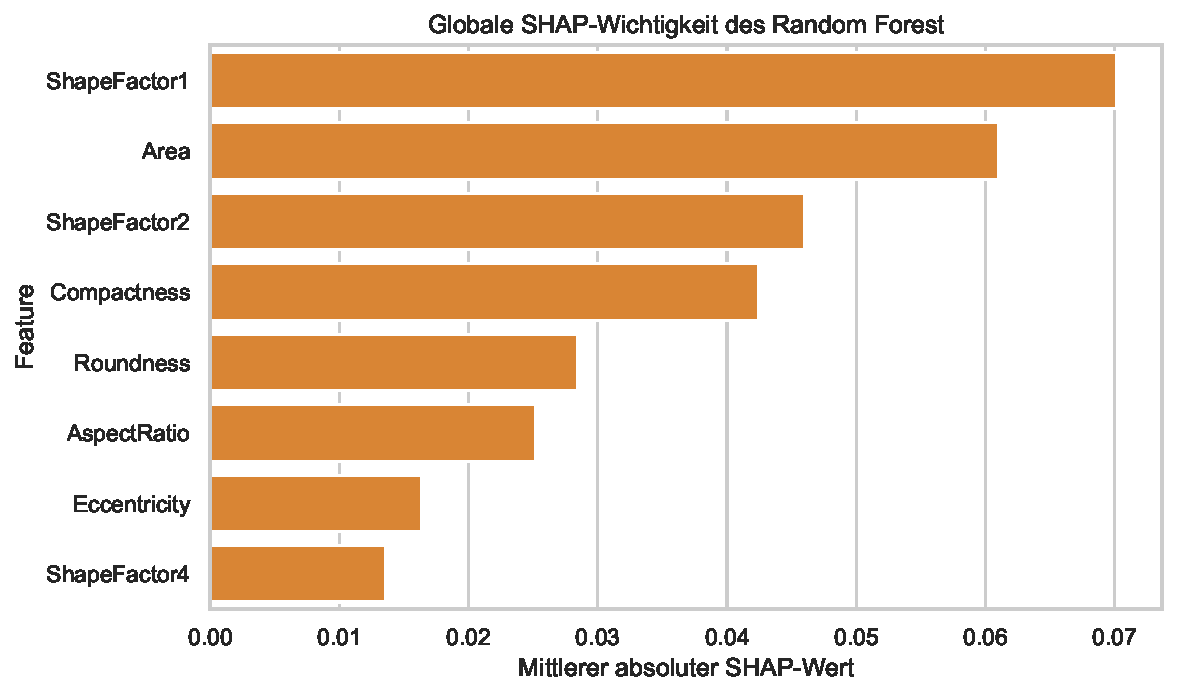
\includegraphics[width=0.85\textwidth]{Graphics/SHAP_Global_RandomForest.pdf}
  \caption{Globale SHAP-Wichtigkeit des Random Forest}
  \label{fig:SHAP_Global_RandomForest}
\end{figure}

Abbildung~\ref{fig:SHAP_Global_RandomForest} bestätigt einen Teil der PFI-Ergebnisse. \texttt{ShapeFactor1} liegt auch bei SHAP an erster Stelle. Danach folgen \texttt{Area}, \texttt{ShapeFactor2} und \texttt{Compactness}. \texttt{Roundness} ist bei SHAP weniger dominant als bei der PFI, bleibt aber im mittleren Bereich. \texttt{ShapeFactor4} liegt in der SHAP-Rangfolge am Ende.

Die Unterschiede zwischen PFI und SHAP sind kein Widerspruch. Beide Methoden messen nicht dasselbe. PFI bewertet, wie stark die Modellleistung fällt, wenn ein Merkmal gestört wird. SHAP misst dagegen die durchschnittliche Größe der Merkmalsbeiträge zur Vorhersage \cite[Kap.~18, Kap.~23]{molnar2025interpretable}. Für die Interpretation ist deshalb vor allem das gemeinsame Muster wichtig: Größen- und Formmerkmale stehen oben, reine Länglichkeitsmaße wie \texttt{AspectRatio} und \texttt{Eccentricity} spielen im erklärten Random Forest eine kleinere Rolle.

\section{Lokale SHAP-Erklärung}

Neben der globalen Sicht wurde eine einzelne korrekt klassifizierte Testbeobachtung betrachtet. Das Modell sagt für diese Beobachtung \texttt{DERMASON} vorher, und die tatsächliche Klasse ist ebenfalls \texttt{DERMASON}. Die lokale SHAP-Erklärung bezieht sich auf genau diese vorhergesagte Klasse.

\begin{figure}[htbp]
  \centering
  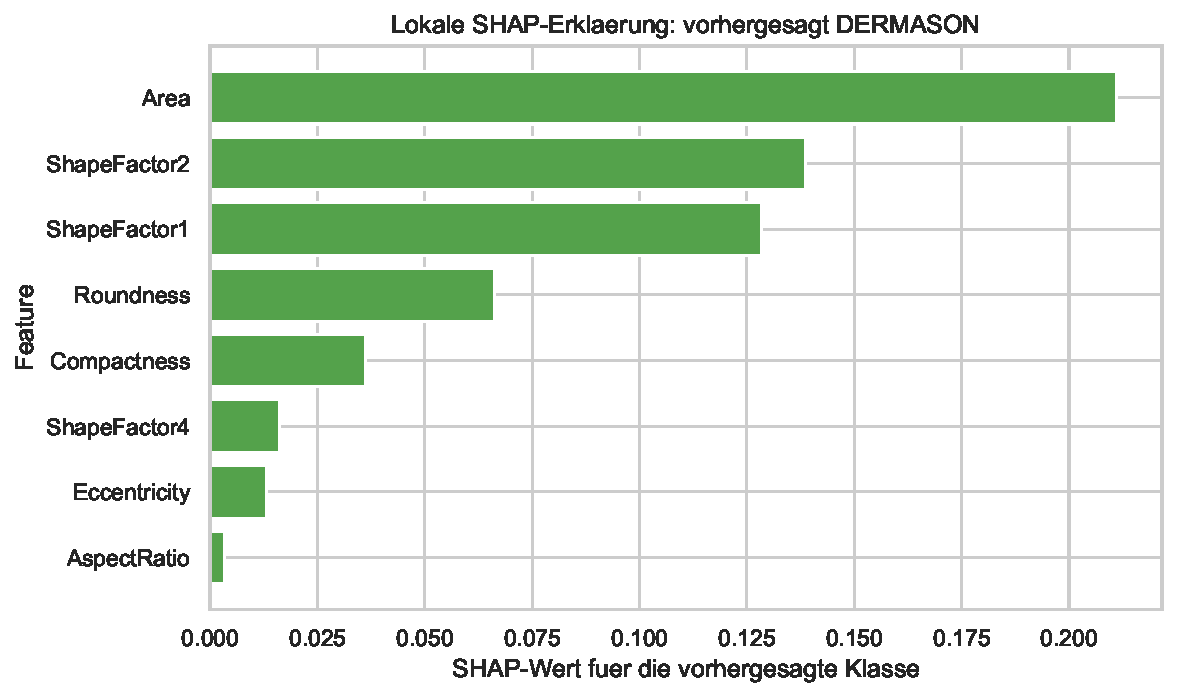
\includegraphics[width=0.85\textwidth]{Graphics/SHAP_Local_RandomForest.pdf}
  \caption{Lokale SHAP-Erklärung einer korrekt klassifizierten DERMASON-Instanz}
  \label{fig:SHAP_Local_RandomForest}
\end{figure}

Abbildung~\ref{fig:SHAP_Local_RandomForest} zeigt, dass vor allem \texttt{Area}, \texttt{ShapeFactor2} und \texttt{ShapeFactor1} die Vorhersage in Richtung \texttt{DERMASON} verschieben. Auch \texttt{Roundness} und \texttt{Compactness} tragen positiv bei, aber schwächer. \texttt{AspectRatio} und \texttt{Eccentricity} haben in diesem konkreten Fall nur geringe Beiträge.

Die Beobachtung passt zur globalen Auswertung. Auch dort stehen \texttt{ShapeFactor1}, \texttt{Area}, \texttt{ShapeFactor2} und \texttt{Compactness} weit oben. Für diesen Fall wirkt die Vorhersage daher nicht zufällig oder von einem schwer erklärbaren Einzelmerkmal abhängig. Das Modell stützt sich auf mehrere geometrische Merkmale, die zur Beschreibung der Bohnenform passen.

\section{Lokale Erklärungen mit LIME}

LIME wurde für dieselbe Testbeobachtung berechnet wie die lokale SHAP-Erklärung. Das erleichtert den Vergleich der Methoden. LIME erzeugt künstliche Varianten der Beobachtung, lässt diese vom Random Forest vorhersagen und trainiert daraus ein lokales Ersatzmodell \cite[Kap.~14]{molnar2025interpretable}. Die erklärten Merkmale erscheinen dabei als Bedingungen, weil kontinuierliche Werte diskretisiert werden.

\begin{figure}[htbp]
  \centering
  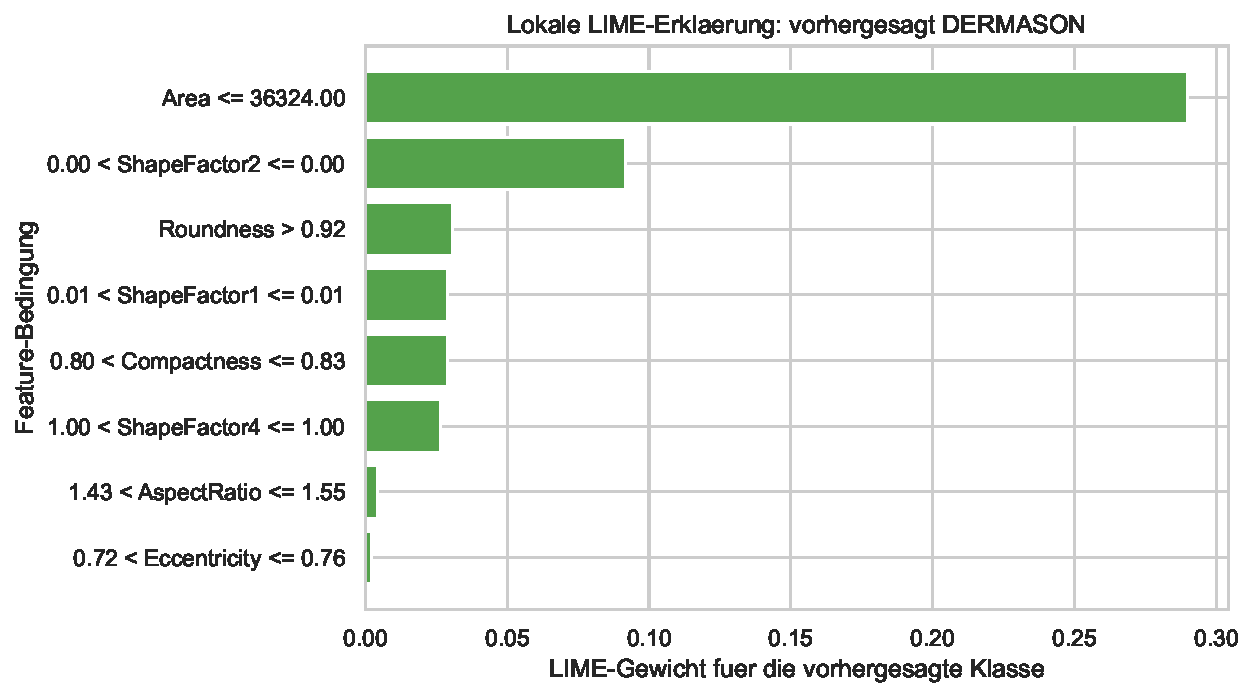
\includegraphics[width=0.85\textwidth]{Graphics/LIME_Local_RandomForest.pdf}
  \caption{Lokale LIME-Erklärung derselben DERMASON-Instanz}
  \label{fig:LIME_Local_RandomForest}
\end{figure}

Abbildung~\ref{fig:LIME_Local_RandomForest} zeigt ebenfalls einen starken Beitrag der Fläche. Die wichtigste LIME-Bedingung lautet: \texttt{Area} ist kleiner oder gleich 36324{,}00. Sie erhält das größte positive Gewicht für die vorhergesagte Klasse \texttt{DERMASON}. Danach folgen Bedingungen zu den Formmerkmalen \texttt{ShapeFactor2}, \texttt{Roundness}, \texttt{ShapeFactor1}, \texttt{Compactness} und \texttt{ShapeFactor4}. \texttt{AspectRatio} und \texttt{Eccentricity} tragen auch bei LIME nur schwach zur lokalen Erklärung bei.

Damit stützt LIME die SHAP-Erklärung für diesen Fall. Beide Methoden heben Größe und Formfaktoren hervor. Die Ergebnisse sollten trotzdem nicht als exakte Kausalbegründung gelesen werden. Molnar beschreibt LIME als lokale Approximation, deren Ergebnis von der gewählten Nachbarschaft, dem Sampling und der Stabilität des Ersatzmodells abhängt \cite[Kap.~14]{molnar2025interpretable}. Für diese Arbeit wird LIME deshalb als ergänzende Plausibilitätsprüfung genutzt, nicht als alleinige Erklärung.

\section{Vergleich der XAI-Methoden}

Die drei Methoden beantworten unterschiedliche Fragen. Permutation Feature Importance zeigt, welche Merkmale für die Testleistung des Random Forest wichtig sind. SHAP zeigt, wie stark Merkmale zu Vorhersagen beitragen, und kann von lokalen Erklärungen zu einer globalen Rangfolge verdichtet werden. LIME erklärt einzelne Vorhersagen über ein lokales Ersatzmodell.

Inhaltlich zeigen die Methoden ein ähnliches Bild. \texttt{ShapeFactor1}, \texttt{Area}, \texttt{ShapeFactor2}, \texttt{Roundness} und \texttt{Compactness} treten wiederholt als wichtige Merkmale auf. Das spricht dafür, dass der Random Forest vor allem Größen- und Forminformationen nutzt. Die beiden Länglichkeitsmerkmale \texttt{AspectRatio} und \texttt{Eccentricity} sind im aktuellen Modell weniger einflussreich.

Die Unterschiede zwischen den Rangfolgen sind trotzdem wichtig. \texttt{Roundness} ist bei der PFI stärker als bei SHAP. \texttt{ShapeFactor2} ist bei SHAP stärker als bei der PFI. Solche Abweichungen sind bei korrelierten Merkmalen erwartbar, weil die Methoden unterschiedliche Größen messen und weil sich Informationen zwischen ähnlichen Merkmalen aufteilen können \cite[Kap.~18, Kap.~23]{molnar2025interpretable}. Die XAI-Ergebnisse sollten daher als gemeinsames Muster gelesen werden, nicht als absolute Rangliste einzelner Variablen.

\section{Zwischenfazit}

Die XAI-Auswertung zeigt, dass der Random Forest seine Entscheidungen vor allem auf morphologisch gut interpretierbare Merkmale stützt. Besonders wichtig sind Formfaktoren, Fläche, Rundheit und Kompaktheit. Damit passen die Erklärungen grundsätzlich zum Domänenwissen: Bohnensorten unterscheiden sich sichtbar durch Größe, Rundheit und Form.

Für die Forschungsfrage bedeutet das: Die Modelle liefern nicht nur hohe Klassifikationswerte, sondern ihre Entscheidungen lassen sich mit den verwendeten XAI-Methoden inhaltlich nachvollziehen. Die Aussage bleibt aber begrenzt. Stark korrelierte Merkmale erschweren die Interpretation, und lokale Erklärungen zeigen immer nur einzelne Fälle. Für die weitere Diskussion ist deshalb entscheidend, die XAI-Ergebnisse zusammen mit der EDA, den Konfusionsmatrizen und den bekannten Fehlermustern zwischen \texttt{DERMASON}/\texttt{SIRA} sowie \texttt{BARBUNYA}/\texttt{CALI} zu lesen.
